\documentclass[11pt]{article}
\usepackage[letterpaper,margin=1in]{geometry}
\usepackage{fontspec}
\setmainfont{Charter}
\setsansfont{Helvetica Neue}
\usepackage{microtype}
\usepackage{booktabs}
\usepackage[table]{xcolor}
\usepackage{titlesec}
\usepackage{enumitem}
\usepackage{fancyhdr}
\usepackage{graphicx}
\usepackage[hidelinks]{hyperref}
\usepackage{xurl}

\definecolor{wolf}{HTML}{CC0000}
\definecolor{inkgray}{HTML}{555555}

\titleformat{\section}{\sffamily\bfseries\Large\color{wolf}}{\thesection}{0.8em}{}[{\color{wolf!60}\vspace{1pt}\titlerule[0.7pt]}]
\titleformat{\subsection}{\sffamily\bfseries\large}{\thesubsection}{0.8em}{}

\pagestyle{fancy}
\fancyhf{}
\fancyhead[L]{\sffamily\footnotesize\color{inkgray}Plan v0 --- AI at NC State CSC}
\fancyhead[R]{\sffamily\footnotesize\color{inkgray}\thepage}
\renewcommand{\headrulewidth}{0.4pt}
\renewcommand{\headrule}{{\color{inkgray!50}\hrule width\headwidth height 0.4pt}}

\setlength{\parskip}{0.4em}
\setlength{\parindent}{0pt}

% evidence-strength tags
\newcommand{\Ecite}{\textsuperscript{\color{wolf}\sffamily\bfseries E1}}   % external published evidence
\newcommand{\Epeer}{\textsuperscript{\color{wolf}\sffamily\bfseries E2}}   % peer-catalog evidence (Appendix A)
\newcommand{\Epos}{\textsuperscript{\color{inkgray}\sffamily\bfseries E3}} % our position; argument, not yet evidence

\begin{document}

{\sffamily\bfseries\huge Plan v0: AI at NC State CSC\par}
\vspace{2pt}
{\sffamily\large\color{inkgray} Win by teaching everyone's AI rigor, cheaply, starting this semester\par}
\vspace{6pt}
{\color{wolf}\rule{\linewidth}{1.4pt}}\\[-2pt]
{\color{wolf!40}\rule{\linewidth}{0.5pt}}
\vspace{4pt}

{\color{inkgray}\sffamily T.~Menzies \quad·\quad August 4, 2026 \quad·\quad internal working memo\\
Evidence tags: \Ecite\ = published/external source \quad \Epeer\ = peer-catalog evidence (Appendix~A) \quad \Epos\ = our position --- argument, weaker support, use with care.\par}
\vspace{0.4em}
{\color{inkgray!50}\rule{\linewidth}{0.4pt}}
{\sffamily\tableofcontents}
\vspace{0.6em}

\section{Situation}

The new Provost has put his agenda in print~[1]: universities are ``built like tanks\ldots yet at this moment, being agile is essential''; AI must be dosed early and redosed through the curriculum; fundamentals are non-negotiable; parsimony --- ``small language models that do bespoke tasks with way less power usage'' --- will transform ``the way we educate''; and the title of the piece is his test: \emph{stop talking, start doing}.\Ecite

Meanwhile every department on NC State's BOG-approved peer list is moving: Purdue ships a BS in AI~[6]; Arizona ships an AI BS and minor~[7]; Duke puts required AI into its CS core in Fall 2026~[8]; Maryland's AI bachelor's degrees arrive 2026--27~[9]; Virginia Tech's all-majors AI minor opened this month~[10].\Epeer\ Our own BS-in-AI is on hold, reconfigured toward a joint ECE/ISE offering, and campus AI policy is set by many people, some of which do not have advanced degrees in CS.\Epos

\section{Diagnosis}

We benchmarked NCSU CSC against all twelve BOG peers, Duke, and an ideal department scored from the Provost's published criteria (Appendix~A; every cell evidence-linked to public catalogs). Two results:

\begin{enumerate}[itemsep=2pt]
\item \textbf{On the Provost's nine curricular constructs, NCSU is already the closest department to his ideal} (tied with Purdue). Year-one applied AI (CSC~201), a thirty-year corporate capstone, live AI concentration and MCS track.\Epeer
\item \textbf{Add two political constructs --- ownership settled vs.\ turf-locked, institutional bet vs.\ no push --- and NCSU falls from 1st to 10th.} NCSU's turf-lock score is the worst in the set.\Epeer\ The deficit is politics, not curriculum. ``Everyone owns AI, so no one is the expert.''\Epos
\end{enumerate}

Conclusion: the ownership war is unwinnable and unnecessary. The winnable claim is \emph{rigor as service}: CS teaches every NC State engineer to test, evaluate, secure, and afford AI. No peer requires such coursework today --- the lane is empty.\Epeer

\section{Why rigor, why us, why now}

Industrial AI has problems that only a computer-science department can teach its way out of:

\begin{itemize}[itemsep=2pt]
\item \textbf{Unsustainable costs.} Current AI API pricing is venture-subsidized; when subsidies end, costs are predicted to rise 10--100$\times$. Microsoft lost \$400B in market value in one week in January 2026; 95\% of enterprise AI apps fail to return revenue.\Ecite~[5] Survival = mixing expensive and cheap methods --- exactly the parsimony the Provost endorsed~[1] and that our EZR results demonstrate (state-of-the-art tabular optimization in $\sim$300 lines, no GPU)~[3].\Ecite
\item \textbf{Poor testing.} 52\% of ChatGPT answers to programming questions contain incorrect information, and humans overlook the errors 39\% of the time; only $\sim$29\% of Copilot suggestions are fully correct; LLMs regenerate known bugs from training data.\Ecite~[5] Testing consumes roughly half of development effort, and ``vibe coding'' defers it into production.\Ecite~[5]
\item \textbf{Workforce deskilling.} If AI writes the junior-engineer code, where do senior engineers come from? The Provost's own version: fundamentals can't be replaced because student brains are ``hardening.''~[1] Our version is stronger and less supported: CS $\neq$ SE $\neq$ bracket matching, and industry's perception says otherwise.\Epos
\item \textbf{Governance, not prompting.} From our faculty draft~[5]: \emph{we do not need classes on how to prompt; we need classes on how to govern} --- oversight, cost--benefit analysis, and empirical monitoring of AI in real systems. This is also an accreditation argument, not just an opinion: ABET Outcomes 2 and 4 (evaluate solutions; informed judgment) and the ACM CS2023 competency model already require students who can \emph{verify} what they cannot hand-write.\Ecite~[5]
\end{itemize}

One line for all of it (faculty consensus~[5]): \textbf{``AI, carefully. AI enthusiasm plus engineering rigor.''}

\section{The plan}

Ranked by friction, lowest first. Items 1--4 need no degree paperwork.

\begin{enumerate}[itemsep=3pt]
\item \textbf{Quit the ownership war; sell rigor as service.} CSC's pitch is the deficit nobody else covers --- testing, evaluation, security, economics of AI systems. A service claim triggers no veto.\Epeer
\item \textbf{Route around high-friction artifacts.} Friction ladder: course-level learning-objective edits $<$ CSC 202/301 service sequence $<$ minor $<$ MS+AI (near-approved --- push it through now; it is the cheap win) $<$ BS (park it; on-hold status is sunk cost).\Epos
\item \textbf{202/301 for all engineering = the resource engine.} Service enrollment $\to$ SCH money $\to$ staff lines. Degrees follow money, not vice versa. This is also precisely the Provost's ``1,850 freshmen'' question answered~[1].\Ecite
\item \textbf{Speak the Provost's language back to him.} His interview supplies the vocabulary --- agility, parsimony, dose-and-redose, stop-talking-start-doing. Our ``Simple Ain't Stupid'' agenda~[3] is the same position with benchmarks. A one-page white paper in his frame, delivered inside his first hundred days: new provosts hunt early wins; hand him one.\Epos
\item \textbf{Demos beat proposals.} Running freshman AI module, CS510 requirements-engineering artifacts, lunch swap-shops, advisory-board and industry letters (Red Hat is already in orbit~[1]) $>$ any committee document.\Epos
\item \textbf{Grab the fellowship program.} The Dean's Applied-AI faculty fellowships exist and are budgeted (first cohort 2026). CSC people in the first cohorts = legitimacy plus allies, no committee required.\Epeer
\item \textbf{Two new subjects, not twenty} (from the faculty draft~[5], which proposed a minimal-impact update): a \emph{management-level subject} on the economic cost--benefit of AI adoption, and a \emph{software-analytics subject} on empirically monitoring AI's true impact on project health. Both feed the empty rigor lane.\Ecite
\item \textbf{Infrastructure asks, priced} (from~[5]): one to two faculty hires in AI financial governance / operational auditing, and a centralized \emph{NC State LLM Token Bank} (\$50--\$500 per student per semester at post-subsidy prices) so courses can teach cost-aware AI for real.\Ecite
\end{enumerate}

\textbf{Blunt version:} we cannot win a vote on ``CS owns AI.'' We can win ``CS teaches everyone's AI rigor, cheaply, starting this semester'' --- and the Provost has already endorsed every ingredient in print.

\newpage
\section*{Appendix A --- The Repertory Grids}

Method: repertory grid (Kelly~[4]). Elements: NCSU CSC, the twelve BOG-approved peers~[2], Duke, and an IDEAL department scored from the Provost's published positions~[1]. Grid~1 constructs derive from the Provost's interview; Grid~1+ appends two constructs elicited from T.~Menzies by triadic comparison (\dag). Cells score 1 (left pole, ideal) to 5 (right pole); labels carry the scale as \emph{1=\ldots 5=\ldots}. $d=\sum_i|x_i-\mathrm{ideal}_i|$. Ward linkage over Euclidean distance; constructs clustered above, departments at right. Every Grid-1 cell has a one-line evidence note and URL in \texttt{repgrid/evidence-grid1.md}; anchors were fixed before scoring (\texttt{repgrid/rubric-grid1.md}).

\begin{center}
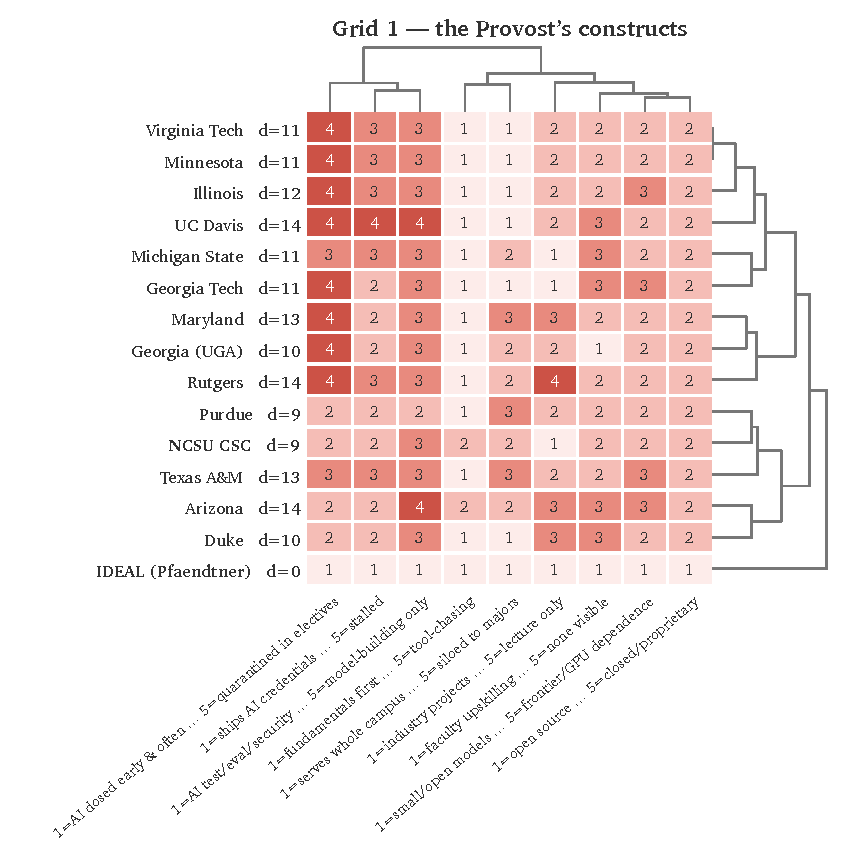
\includegraphics[width=\linewidth]{repgrid/grid1-cluster.pdf}
\end{center}

\subsection*{Grid 1 findings}
\begin{enumerate}[itemsep=2pt]
\item By the Provost's own criteria, NCSU is the closest department to his ideal (tied with Purdue, $d=9$).
\item Early AI dosing is the sector-wide failure: nine of fourteen departments require no AI before senior electives.
\item AI systems rigor (testing/eval/security) is an empty lane: no department requires it; first mover defines the category.
\item Fundamentals offer no differentiation; the whole sector is strong there.
\end{enumerate}

\begin{center}
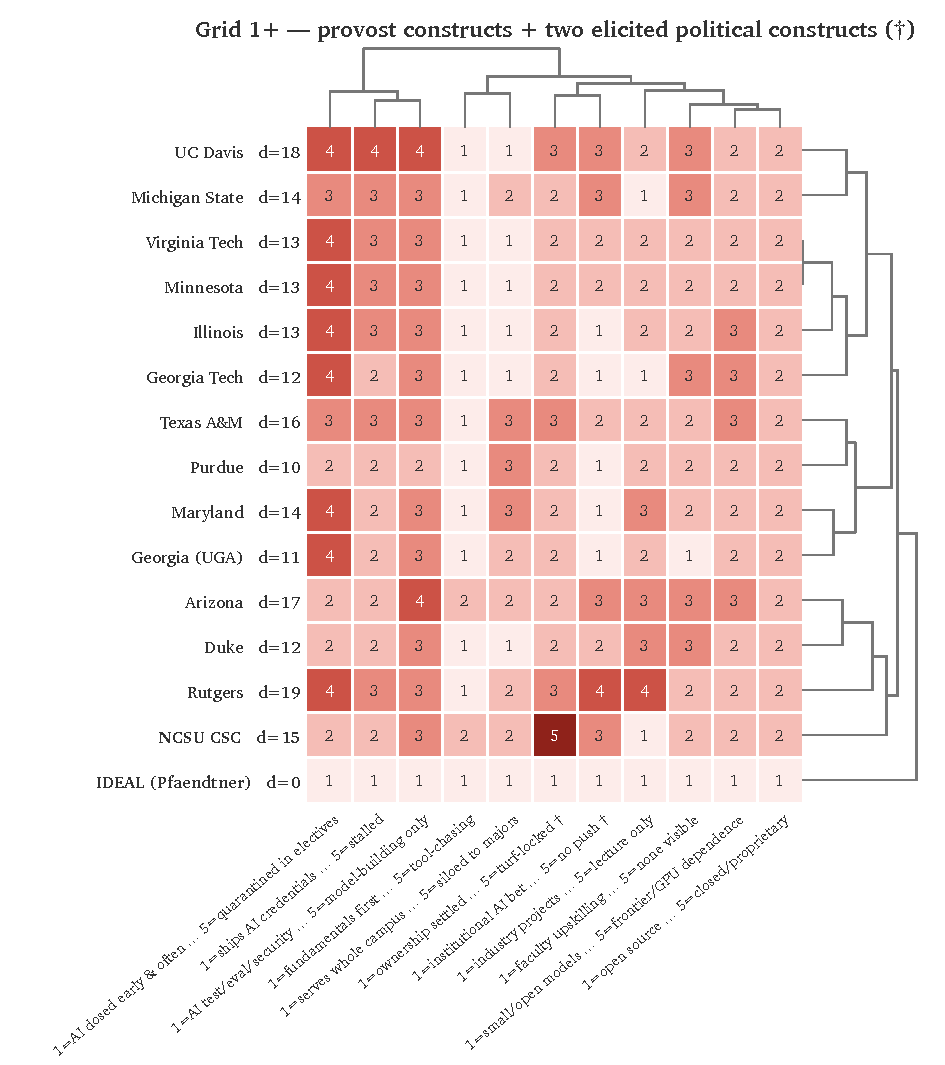
\includegraphics[width=\linewidth]{repgrid/grid1aug-cluster.pdf}
\end{center}

\subsection*{Grid 1+ findings}
\begin{enumerate}[itemsep=2pt]
\item Two political constructs cost NCSU nine places: first ($d=9$) on curricular substance; tenth ($d=15$) once turf-lock (worst in set) and institutional-bet enter. The entire drop is politics.
\item One elicited belief failed its evidence check: UC~Davis, construed as having ``shipped AI degrees,'' has shipped nothing (AI major/minor still at survey stage). Purdue is the lone shipping benchmark.
\item Both lenses agree on two things: shipping credentials and cross-campus reach. Safe load-bearing claims for any public document.
\item Prescription follows the arithmetic: fix ownership and visible commitment, not curriculum --- exit the turf fight via service teaching; attach to funded institutional signals (fellowships, applied-AI initiative).
\end{enumerate}

\subsection*{Construct rubric (anchors fixed before scoring)}

{\footnotesize\renewcommand{\arraystretch}{1.25}
\begin{tabular}{@{}p{0.7cm}p{4.6cm}p{4.6cm}p{4.9cm}@{}}
\toprule
& \textbf{Score 1 anchor} & \textbf{Score 5 anchor} & \textbf{Source}\\
\midrule
C1 & required AI touchpoint in year 1, reinforced in $\geq$2 later required courses & AI reachable only via senior/grad electives & Pfaendtner: ``where does the dose of AI come early on\ldots keep redosing it''~[1, p.\,10]\\
C2 & theory/algorithms required before tool use & vendor-tool/prompting-led curriculum & ``can't replace the time\ldots to learn fundamentals''~[1, p.\,10]\\
C3 & courses run small/local/open models, cost-aware & paid frontier APIs / large clusters & ``parsimony---small language models\ldots the way we educate''~[1, p.\,17]; EZR~[3]\\
C4 & required projects with external/industry clients & lecture/exam dominant & title ``Stop talking, start doing''~[1]\\
C5 & open tools required; public course repos & proprietary stack, closed materials & ``open source means we publish our work first''~[1, p.\,13--14]\\
C6 & named faculty AI-upskilling program & none visible & faculty fellowship program~[1, p.\,11]\\
C7 & CS-run AI service courses/minor open to all majors & AI restricted to CS majors & 1,850 freshmen---``How are we teaching them to think about AI?''~[1, p.\,9]\\
C8 & AI BS + minor + MS live and enrolling & no AI-named credential & ``being agile is essential''~[1, p.\,9]\\
C9 & required testing/eval/security-of-AI coursework & model-building content only & faculty draft~[5]; Pfaendtner--Griffin exchange~[1, p.\,10]\\
C10\dag & one unit clearly owns AI credentials; campus accepts & proposals blocked/reconfigured by inter-unit contest & elicited, triad 5; scored from dossier ownership facts\\
C11\dag & named university AI investment with money & no visible institutional AI investment & elicited, triad 6; scored from dossier partnership evidence\\
\bottomrule
\end{tabular}}

\vspace{4pt}
{\color{inkgray}\footnotesize Score 3 = midpoint. No-public-signal cells score 3 and are flagged, never silently guessed. IDEAL scores 1 everywhere. Retired elicited constructs: brand (duplicates public rankings), land-grant status (constant across public peers).}

\newpage
\subsection*{References}
\begin{enumerate}[itemsep=2pt,label={[\arabic*]}]
\item S.~Griffin (interviewer), ``Stop talking, start doing: how universities rise to the challenge of the AI revolution.'' Interview with NC State Provost Jim Pfaendtner. \emph{Red Hat Research Quarterly}, Vol.~8.1, Summer 2026, ISSN 2691-5278. \url{https://research.redhat.com/blog/article/stop-talking-start-doing-how-universities-rise-to-the-challenge-of-the-ai-revolution/}
\item UNC System Office, ``2025 UNC Peer Institution Study,'' approved by the Board of Governors May 15, 2025. \url{https://isa.ncsu.edu/facts-comparisons/peer-universities/}
\item T.~Menzies and S.~Srinivasan, ``Can AI be Easy? Lessons Learned from the EZR.py Toolkit,'' 2026. \url{https://arxiv.org/pdf/2606.03640}
\item G.~A. Kelly, \emph{The Psychology of Personal Constructs}, Norton, 1955.
\item M.~d'Amorim, W.~Assunção, S.~Heckman, S.~Kuttal, T.~Menzies, J.-P.~Ore, K.~Stolee, B.~Xu, ``Restoring `Engineering' to Software Engineering,'' NC State CSC faculty working draft, August 2026 (internal; sources for the cost/testing statistics are cited therein).
\item Purdue University, ``Bachelor of Science in Artificial Intelligence,'' Dept.\ of Computer Science degree requirements, accessed Aug.\ 2026. \url{https://www.cs.purdue.edu/undergraduate/curriculum/bachelor-ai.html}
\item University of Arizona, ``B.S.\ in Artificial Intelligence'' and ``Artificial Intelligence Minor,'' accessed Aug.\ 2026. \url{https://cs.arizona.edu/aibs}; \url{https://catalog.arizona.edu/programs/AIMINU}
\item Duke University, ``BS Degree Requirements (Fall 2026 and beyond): COMPSCI 270 + AI core course,'' Dept.\ of Computer Science, accessed Aug.\ 2026. \url{https://cs.duke.edu/undergraduate/degrees/BS}
\item University of Maryland AIM Institute, ``UMD to Launch 2 Bachelor's Degrees [in AI],'' 2026 (BA Fall 2026, BS Fall 2027). \url{https://aim.umd.edu/news-events/news/umd-launch-2-bachelors-degrees-explore-technical-human-dimensions-ai}
\item Virginia Tech, ``Artificial Intelligence Minor'' (declarable from Aug.\ 3, 2026; open to all majors), University Catalog. \url{https://catalog.vt.edu/undergraduate/minors/artificial-intelligence-minor/}
\end{enumerate}

\end{document}
